\section{Design / Implementation}
\label{ch:impl}
\noindent	

This chapter aims to discuss the implementation details of the system presented in \textit{figure~\ref{system-overview}}.

\subsection{CoAP server}

\begin{figure}[H]
	\begin{center}
		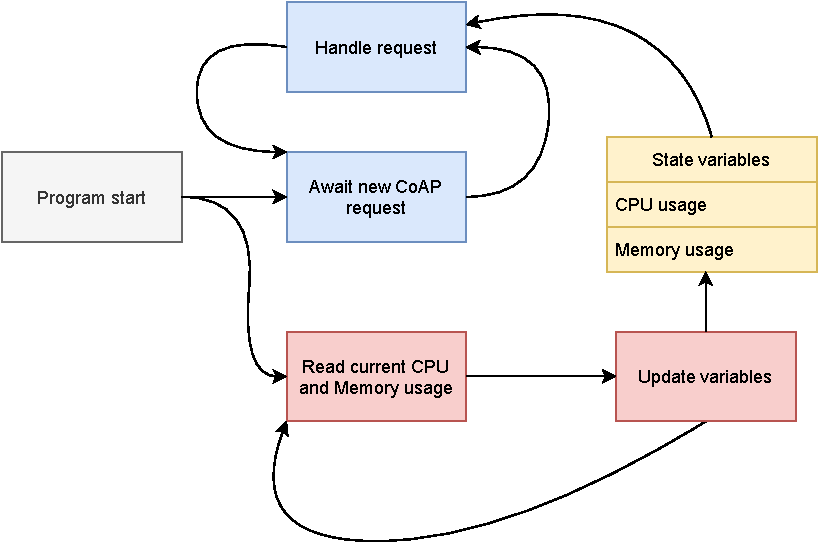
\includegraphics[width=\textwidth]{./doc/coap_flowchart.pdf}
		\caption{Flowchart depicting the duties and the program flow of the CoAP server.}
		\label{coap-figure}
	\end{center}
\end{figure}

\textit{Figure~\ref{coap-figure}} shows the program flow of the CoAP server. The flow is separated into two threads marked as blue and red boxes in figure~\ref{coap-figure}. There is also a yellow box, representing data shared between the threads. This data is locked behind mutex locks so as to not cause any race conditions between the red and blue thread. 

The red thread is responsible for regularly reading the current CPU and memory usage from the system. It then tries to access the shared state variables in order to update them with the new information. Upon successfully updating the variables, the lock is released and the thread sleeps for one second before attempting to read the CPU and memory usage once more.

The blue thread is responsible for performing all server-related duties of the system component. It listens for potential requests to the urls \lstinline{/cpu} and \lstinline{/mem}. Upon recieving a request, it tries to access the corresponding shared state variable, embeds it into a response, and sends the response. It then goes back into listening mode, awaiting the next request.

\subsection{CoAP + MQTT Client}

\begin{figure}[H]
	\begin{center}
		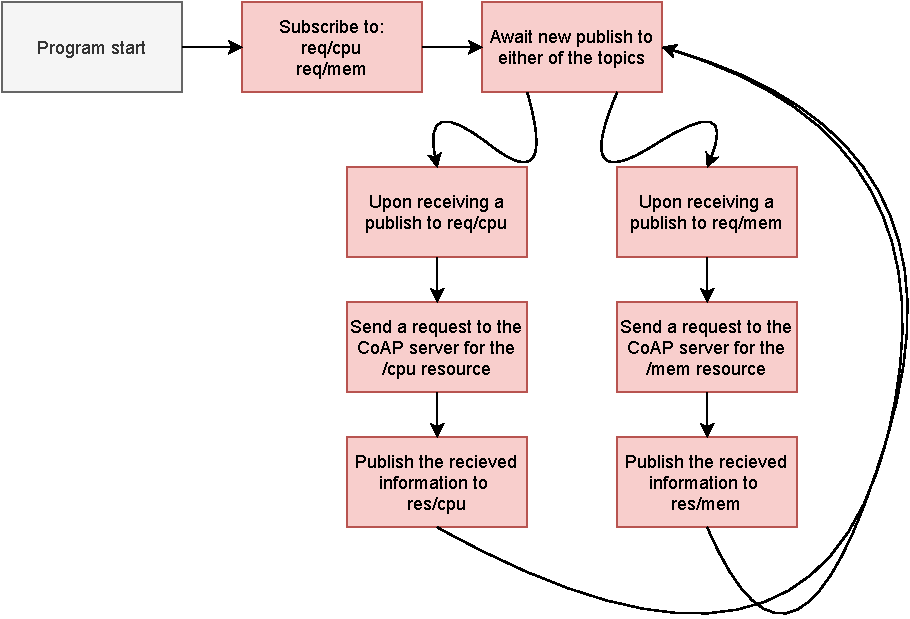
\includegraphics[width=\textwidth]{./doc/coap_mqtt_flowchart.pdf}
		\caption{Flowchart depicting the program flow of the CoAP + MQTT Client component} 
		\label{coap-mqtt}
	\end{center}
\end{figure}

The CoAP + MQTT Client, pictured in \textit{figure~\ref{coap-mqtt}} can be viewed as a sort of bridge between the two protocols. Its only purpose is to intercept publications to the \lstinline{res/cpu} and \lstinline{req/cpu} MQTT topics. Upon receiving a message from either of those two topics, a request to the CoAP server for either the \lstinline{/cpu} or \lstinline{/mem} resource is sent. Once the response to this message is received, the contents thereof is published to either the \lstinline{res/cpu} or the \lstinline{res/mem} topic. Once a publication has been properly handled, the bridge goes back into awaiting a new publication.

\subsection{MQTT Broker}

\begin{figure}[H]
	\begin{center}
		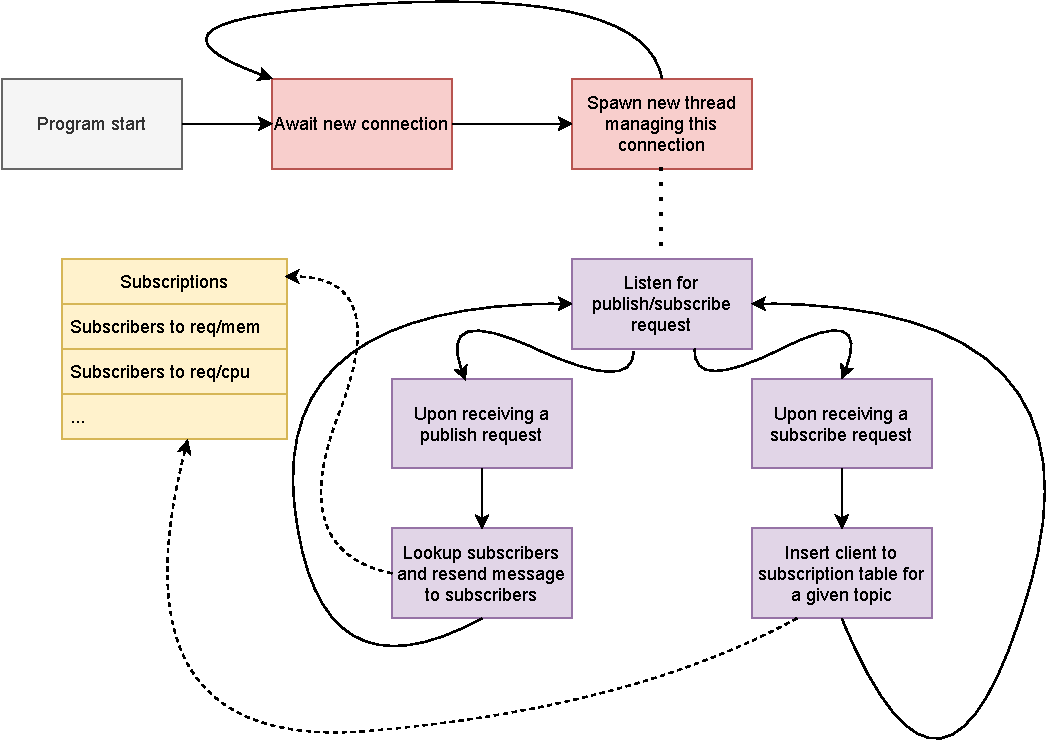
\includegraphics[width=\textwidth]{./doc/mqtt_flowchart.pdf}
		\caption{Flowchart depicting the program flow of the MQTT broker}
		\label{mqtt-broker}
	\end{center}
\end{figure}

The MQTT broker, pictured in \textit{figure~\ref{mqtt-broker}}, is responsible for managing all MQTT topic subscriptions and publications within the system. On startup, it consists solely of one main thread which listens to new connection requests. Once a new connection request is received, a new thread is spawned which maintains this individual client's publish/subscribe messages. All subscriptions are kept track of in a table which maps topic names to a set of clients, meaning that when a new subscription is requested, the client authoring this subscription is inserted into the corresponding set. If a client sends a publish message, a map lookup is performed to find the appropriate set of subscribers, who will then receive a duplicate of the original message.

\subsection{MQTT Client + WebSocket server}

\begin{figure}[H]
	\begin{center}
		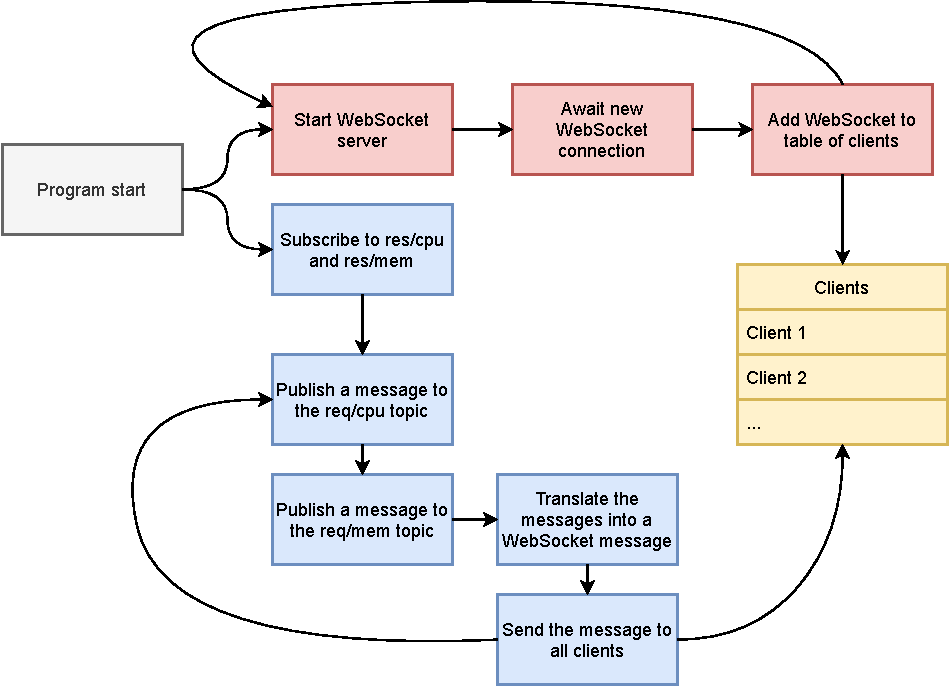
\includegraphics[width=\textwidth]{./doc/mqtt_ws_flowchart.pdf}
		\caption{Flowchart depicting the program flow of the MQTT client + WebSocket server}
		\label{mqtt-ws}
	\end{center}
\end{figure}

The component pictured in \textit{figure~\ref{mqtt-ws}} is responsible for managing the connection between the MQTT broker and the frontend. It achieves this by managing a WebSocket connection to the frontend as well as creating a MQTT client which subscribes to the same broker as the rest of the system. The WebSocket subset of this system is marked in red in \textit{figure~\ref{mqtt-ws}}, whereas the MQTT subset of the system is marked in blue. Both subsystems are run in separate threads, but the list of active clients is indirectly shared between the two subsystems. The WebSocket server thread only manages a set of active clients, appending them to a list as they connect. The MQTT client thread subscribes to the \lstinline{res/cpu} and \lstinline{res/mem} topics, before publishing an empty message to the \lstinline{req/cpu} and \lstinline{req/mem} topics (sequentially). Before the requests are sent, a timestamp is made. Another timestamp is made when the response is received. Upon receiving both responses, the difference between the timestamps is averaged before being placed into a JSON string which also contains the measured CPU usage and the measured memory usage; This string is embedded into a WebSocket message, which is distributed to all active clients. 

\subsubsection{The WebSocket protocol}

In order to implement the above component, it was of interest to look into the WebSocket protocol specification and implement pieces of it. These pieces include:

\begin{itemize}
	\item Parsing the client handshake request
	\item Creating a valid handshake response
	\item Encoding/decoding of data frames
\end{itemize}

\begin{figure}[H]
	\begin{center}
		\begin{lstlisting}
GET /chat HTTP/1.1
Host: example.com:8000
Upgrade: websocket
Connection: Upgrade
Sec-WebSocket-Key: dGhlIHNhbXBsZSBub25jZQ==
Sec-WebSocket-Version: 13
		\end{lstlisting}
		\caption{An example of the client handshake request performed when a WebSocket client wishes to connect to a server\cite{ws-howto}.}
		\label{handshake-request}
	\end{center}
\end{figure}

Parsing the client handshake request (see \textit{figure~\ref{handshake-request}}) is a rather trivial problem. It closely resembles the HTTP header format in how several key-value pairs are presented as one big string, making the headers easy to read for humans. The important parts to extract is both the intent of using the WebSocket protocol, but also the \lstinline{Sec-WebSocket-Accept}-header. The value associated with this header needs to be extracted in order to formulate a valid response header. After extracting the key, the correct accept key is generated by\cite{ws-howto}:

\begin{enumerate}
	\item Concatenate the key with the magic string: \\
		\lstinline{258EAFA5-E914-47DA-95CA-C5AB0DC85B11}.
	\item Calculate the SHA-1 hash of this new string.
	\item base64 encode the hash into a new string.
	\item The encoded hash is the accept key.
\end{enumerate}

After the accept key has been created, the handshake response can be created. An example of such a response is shown in \textit{figure~\ref{handshake-response}}.

\begin{figure}[H]
	\begin{center}
		\begin{lstlisting}
HTTP/1.1 101 Switching Protocols
Upgrade: websocket
Connection: Upgrade
Sec-WebSocket-Accept: s3pPLMBiTxaQ9kYGzzhZRbK+xOo=
		\end{lstlisting}
		\caption{An example of the server handshake response performed when a WebSocket server wishes to accept a client\cite{ws-howto}.}
		\label{handshake-response}
	\end{center}
\end{figure}

With the WebSocket handshake underway, all that is left is the ability to understand individual WebSocket messages, usually referred to as ''frames''\cite{ws-howto}.

\begin{figure}[H]
	\begin{center}
		\begin{lstlisting}[language=smalltext]
  0                   1                   2                   3
  0 1 2 3 4 5 6 7 8 9 0 1 2 3 4 5 6 7 8 9 0 1 2 3 4 5 6 7 8 9 0 1
 +-+-+-+-+-------+-+-------------+-------------------------------+
 |F|R|R|R| opcode|M| Payload len |    Extended payload length    |
 |I|S|S|S|  (4)  |A|     (7)     |             (16/64)           |
 |N|V|V|V|       |S|             |   (if payload len==126/127)   |
 | |1|2|3|       |K|             |                               |
 +-+-+-+-+-------+-+-------------+ - - - - - - - - - - - - - - - +
 |     Extended payload length continued, if payload len == 127  |
 + - - - - - - - - - - - - - - - +-------------------------------+
 |                               |Masking-key, if MASK set to 1  |
 +-------------------------------+-------------------------------+
 | Masking-key (continued)       |          Payload Data         |
 +-------------------------------- - - - - - - - - - - - - - - - +
 :                     Payload Data continued ...                :
 + - - - - - - - - - - - - - - - - - - - - - - - - - - - - - - - +
 |                     Payload Data continued ...                |
 +---------------------------------------------------------------+
		\end{lstlisting}
		\caption{A slimmed down explanation of how a WebSocket frame is constructed, courtesy of Mozilla Developer Network\cite{ws-howto}.}
		\label{ws-frame}
	\end{center}
\end{figure}

All of the information presented in \textit{figure~\ref{ws-frame}} is not necessary to digest for the project, as the WebSocket server only needs to be able to distribute messages, not necessarily receive them. The \lstinline{opcode} field specifies what the type of the message is. It could be ''binary'', ''text'' or a more specific message, such as ''close''\cite{ws-howto}. The \lstinline{Payload len} fields are partially optional, depending on the message length\cite{ws-howto}. There is also a \lstinline{MASK} bit present in the second byte, which specifies whether the payload is masked using a masking key\cite{ws-howto}. The masking key is the 4 bytes between the end of the payload length field and the actual payload data. The mask is applied by applying the XOR operator on each key-byte and payload-byte pair, cyclically\cite{ws-howto}. The client is required to set the mask bit, but the server does not need to mask its response(s), according to the specification\cite{ws-howto}.

\subsection{HTML/JS frontend}

\begin{figure}[H]
	\begin{center}
		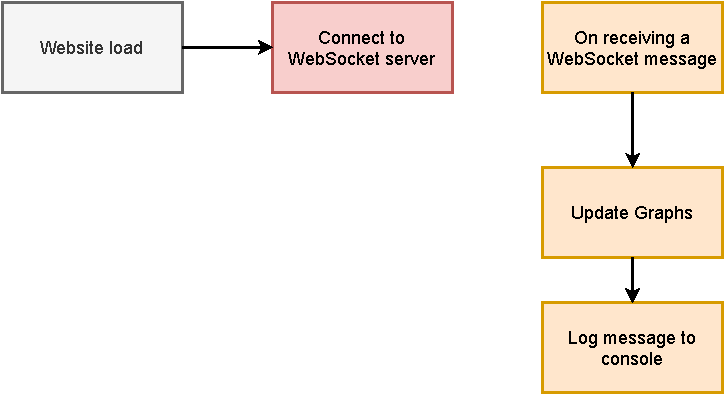
\includegraphics[width=\textwidth]{./doc/html_js_frontend.pdf}
		\caption{Flowchart depicting the ''flow'' of the frontend website}
		\label{html-frontend}
	\end{center}
\end{figure}

As pictured in \textit{figure~\ref{html-frontend}}, the website logic is not particularly interesting. On page load, it tries to establish a connection to the WebSocket server. From there on, it listens to any potential messages and once upon receiving a suitable message, updates the three graphs present on the website. The graphs are meant to present the information of interest, CPU usage, memory usage, and round trip time.

\iffalse
The Design or Implementation chapter often appears in technical reports, but not always in scientific reports. Here, the analysis of the problem is implemented and a technical requirement specification is formulated. At this stage, the most important principles in the suggested alternatives for solution are described and formulated in preparation for evaluation at a later point in the report. The description is sometimes placed before, but generally after the methodology/model chapter, if included at all.

The reader is seldom interested in extremely detailed documentation of computer program code, algorithms, electrical circuit diagrams, user guidance, etc. Such details are placed in the appendices.

As mentioned in the Introduction chapter you have during earlier studies mainly worked with small well defined tasks that have taken minutes or as most hours to solve. In comparison an exam work or a project course can sometimes appear to be an almost overwhelming amount of information because it is so extensive, and this may cause anxiety with regards to where to start. One way to facilitate big projects is to use the top-down-method, i.e. to divide the problem or the structure into smaller problem parts or system parts, and to state specification of  requirements, problem analysis and proposed solution for each part. Eventually small and concrete information will have been identified with similar characteristics to those found in your previous studies.

It is not always practically possible to apply the top-down-method, since the problem may be too complex and initially very difficult to visualise the complete overview. It might prove necessary to alternate between the top-down - and bottom-up-method. The latter means that you start with parts already known to you and from simple problems that have been tackled previously you  make use of that knowledge for aspects that you expect to resolve at a later stage in the project. Gradually increase these parts into the bigger systems and problems and then pursue the direction of project's objective.

The top-down-method has the advantage of giving the report a solid structure, which makes it easier for the reader. The documentation therefore often follows the top-down-method. It is thus possible to divide the structure part into several chapters, and to name them after each problem part and system part, i.e. “Specification of requirements”, “Algorithms”, “User interface”, “Program documentation”, “Prototype” and “Implementation”.
\fi
